\documentclass{article}

\usepackage{tikz}
\usepackage{verbatim}
\usepackage{parskip}
\usepackage{amsthm}
\usepackage{xpatch}
\usepackage{amsmath}
\usepackage{graphicx}

\graphicspath{ {./img/} }

\setlength\parindent{0pt}

\newtheorem{definicija}{Definicija}[subsection]
\newtheorem{lema}{Lema}[subsection]
\newtheorem{izrek}{Izrek}[subsection]
\newtheorem{trditev}{Trditev}[subsection]
\newtheorem{posledica}{Posledica}[subsection]
\newtheorem{domneva}{Domneva}[subsection]
\newtheorem{primer}{Primer}[subsection]
\newtheorem{opomba}{Opomba}[subsection]

\makeatletter
\xpatchcmd{\@thm}{\thm@headpunct{.}}{\thm@headpunct{:}}{}{}
\makeatother

\begin{document}
\pagestyle{empty}

\begin{comment}
definitions
\end{comment}

%%%%%%%%%%%%%%%%%%%%%%%%%%%%%%%%%%%%%%%%%%%%%%%%%%%%%%%%%%%%%%%%%
\section{ Odstotki }

\subsection{ Odstotki in promili }

\begin{definicija}[Procent / odstotek]
    Ulomek $\frac{1}{100}$ pomeni 1 del od 100. Ta delež zapišemo tudi kot $1\%$ in beremo "1 odstotek" (procent). Zapis $p\%$ pomeni $p$ delov od 100 oziroma zapisano z ulomkom $p\% = \frac{p}{100}$.
\end{definicija}


\begin{definicija}[Promil / odtisoček]
    Ulomek $\frac{1}{1000}$ pomeni 1 del od 1000. Ta delež zapišemo tudi kot  $1$\textperthousand\ in beremo "1 promil". Zapis $p$\textperthousand\ pomeni $p$ delov od 1000 oziroma zapisano z ulomkom $p$\textperthousand\ $ = \frac{p}{1000}$.
\end{definicija}

\subsection{Enačba deležev}
\begin{align*}
    \frac{\text{Del celote}}{\text{Celota}} &= \frac{p}{100} = p \%
\end{align*}

\pagebreak
\subsection{ Računanje odstotkov }
Radi bi izračunali koliko je odstotni delež, če je celota 60 in del celote 36.

Izpeljava enačbe za odstotni delež:
\begin{align*}
    \frac{\text{Del celote}}{\text{Celota}} &= \frac{p}{100} = p\% \\
    p\% &= \frac{\text{Del celote}}{\text{Celota}} \quad / \cdot 100\% = \frac{100}{100}\\
    p\% &= \frac{\text{Del celote}}{\text{Celota}} \cdot 100\%\\
\end{align*}

Računanje odstotkov:
\begin{align*}
    p\% &= \frac{\text{Del celote}}{\text{Celota}} \cdot 100\%\\
    p\% &= \frac{36}{60} \cdot 100\%\\
    p\% &= \frac{3}{5} \cdot \frac{100}{1}\% \\
    p\% &= \frac{3 \cdot 20}{1} \%\\
    p\% &= 60\%.
\end{align*}

% \pagebreak
Reševanje s sklepanjem:
\begin{center}
    \begin{tabular}{ c c c c c c}
        % &&&&&  \\
        % Del celote && Odstotek && Ulomek  \\
        &&&&&  \\
        60 & \dots\dots & 100\% & = & $\frac{1}{1}$\\ 
        &&&&&  $:60$ \\
        1 & \dots\dots & $\frac{100}{60}\%=\frac{5}{3}\%$ & = & $\frac{1}{60}$\\ 
        &&&&&  $\cdot 36$\\
        36 & \dots\dots & $\frac{5 \cdot 36}{3}\%=5\cdot12\%=60\%$ & = & $\frac{36}{60} = \frac{3}{5}$\\ 
        &&&&  \\
    \end{tabular}
\end{center}

Reševanje s križnim računom:
\begin{center}
    \begin{tabular}{ c c c  }
        && \\
        60 & \dots\dots & 100\% \\ 
        && \\
        36 & \dots\dots & x\% \\ 
        && \\
    \end{tabular}
\end{center}

\begin{align*}
    x\% = \frac{36 \cdot 100}{60}\% = \frac{3 \cdot 100}{5}\% = \frac{3 \cdot 20}{1}\% = 60\%.
\end{align*}

\pagebreak
\subsection{ Računanje dela celote }
Radi bi izračunali koliko je $27\%$ od $500$ ($27\% = \frac{27}{100} = 0,27$).

Izpeljava enačbe za računanje dela celote:
\begin{align*}
    \frac{\text{Del celote}}{\text{Celota}} &= \frac{p}{100} = p\% \\
    \text{Del celote} &= \frac{p}{100} \cdot \text{Celota}
\end{align*}

Računanje dela celote z ulomki:
\begin{align*}
    27\% \text{ od } 500 &= \frac{27}{100} \cdot 500 = \frac{27}{100} \cdot \frac{500}{1} = \frac{27 \cdot 500}{100 \cdot 1} = \frac{27 \cdot 5}{1} = \frac{135}{1} = 135.
\end{align*}
Računanje dela celote decimalnim zapisom:
\begin{align*}
    27\% \text{ od } 500 &= 0,27 \cdot 500 = 135.
\end{align*}

Reševanje s sklepanjem:
\begin{center}
    \begin{tabular}{ c c c c c c c c }
        % &&&&&&&  \\
        % Del celote && Odstotek && Ulomek && Decimalno  \\
        &&&&&&&  \\
        500 & \dots\dots & 100\% & = & $\frac{1}{1}$ & = & 1\\ 
        &&&&&&&  $:100$ \\
        5 & \dots\dots & 1\% & = & $\frac{1}{100}$ & = & 0,01\\ 
        &&&&&&&  $\cdot 27$\\
        135 & \dots\dots & 27\% & = & $\frac{27}{100}$ & = & 0,27\\ 
        &&&&&&&  \\
    \end{tabular}
\end{center}

Reševanje s križnim računom:
\begin{center}
    \begin{tabular}{ c c c  }
        && \\
        500 & \dots\dots & 100\% \\ 
        && \\
        x & \dots\dots & 27\% \\ 
        && \\
    \end{tabular}
\end{center}

\begin{align*}
    x = \frac{500 \cdot 27}{100} = \frac{5 \cdot 27}{1} = 5 \cdot 27 = 135.
\end{align*}

\pagebreak
\subsection{ Računanje celote }
Radi bi izračunali koliko je celota, če je $80\%$ od celote enako $24$ ($80\%=\frac{80}{100}=\frac{4}{5}=0,8$).

Izpeljava enačbe za računanje celote:
\begin{align*}
    \frac{\text{Del celote}}{\text{Celota}} &= \frac{p}{100} = p\% \\
    \frac{\text{Celota}}{\text{Del celote}} &= \frac{100}{p} \\
    \text{Celota} &= \frac{100}{p} \cdot \text{Del celote}
\end{align*}

Računanje celote z ulomki:
\begin{align*}
    80\% \text{ od } x &= 24 \\
    \frac{80}{100} \cdot x &= 24 \\
    \frac{4}{5} \cdot x &= 24 \quad\quad\ /\cdot5\\
    4 \cdot x &= 24 \cdot 5 \quad /:4\\
    x &= \frac{24 \cdot 5}{4} \\
    x &= \frac{6 \cdot 5}{1} \\
    x &= 30 \\
\end{align*}

Računanje celote z decimalnim zapisom:
\begin{align*}
    80\% \text{ od } x &= 24 \\
    0,8 \cdot x &= 24 \quad /:0,8\\
    x &= 24 : 0,8\\
    x &= 240 : 8\\
    x &= 30 \\
\end{align*}

\pagebreak
Reševanje s sklepanjem:
\begin{center}
    \begin{tabular}{ c c c c c c c c }
        % &&&&&&&  \\
        % Del celote && Odstotek && Ulomek && Decimalno  \\
        &&&&&&&  \\
        24 & \dots\dots & 80\% & = & $\frac{80}{100}$ & = & 0,8\\ 
        &&&&&&&  $:80$ \\
        0,3 & \dots\dots & 1\% & = & $\frac{1}{100}$ & = & 0,01\\ 
        &&&&&&&  $\cdot 100$\\
        30 & \dots\dots & 100\% & = & $\frac{100}{100}$ & = & 1\\ 
        &&&&&&&  \\
    \end{tabular}
\end{center}

Reševanje s križnim računom:
\begin{center}
    \begin{tabular}{ c c c  }
        && \\
        24 & \dots\dots & 80\% \\ 
        && \\
        x & \dots\dots & 100\% \\ 
        && \\
    \end{tabular}
\end{center}

\begin{align*}
    x = \frac{100 \cdot 24}{80} = \frac{5 \cdot 24}{4} = \frac{5 \cdot 6}{1} = 5 \cdot 6 = 30.
\end{align*}

% \pagebreak
% \begin{figure}[h]
%     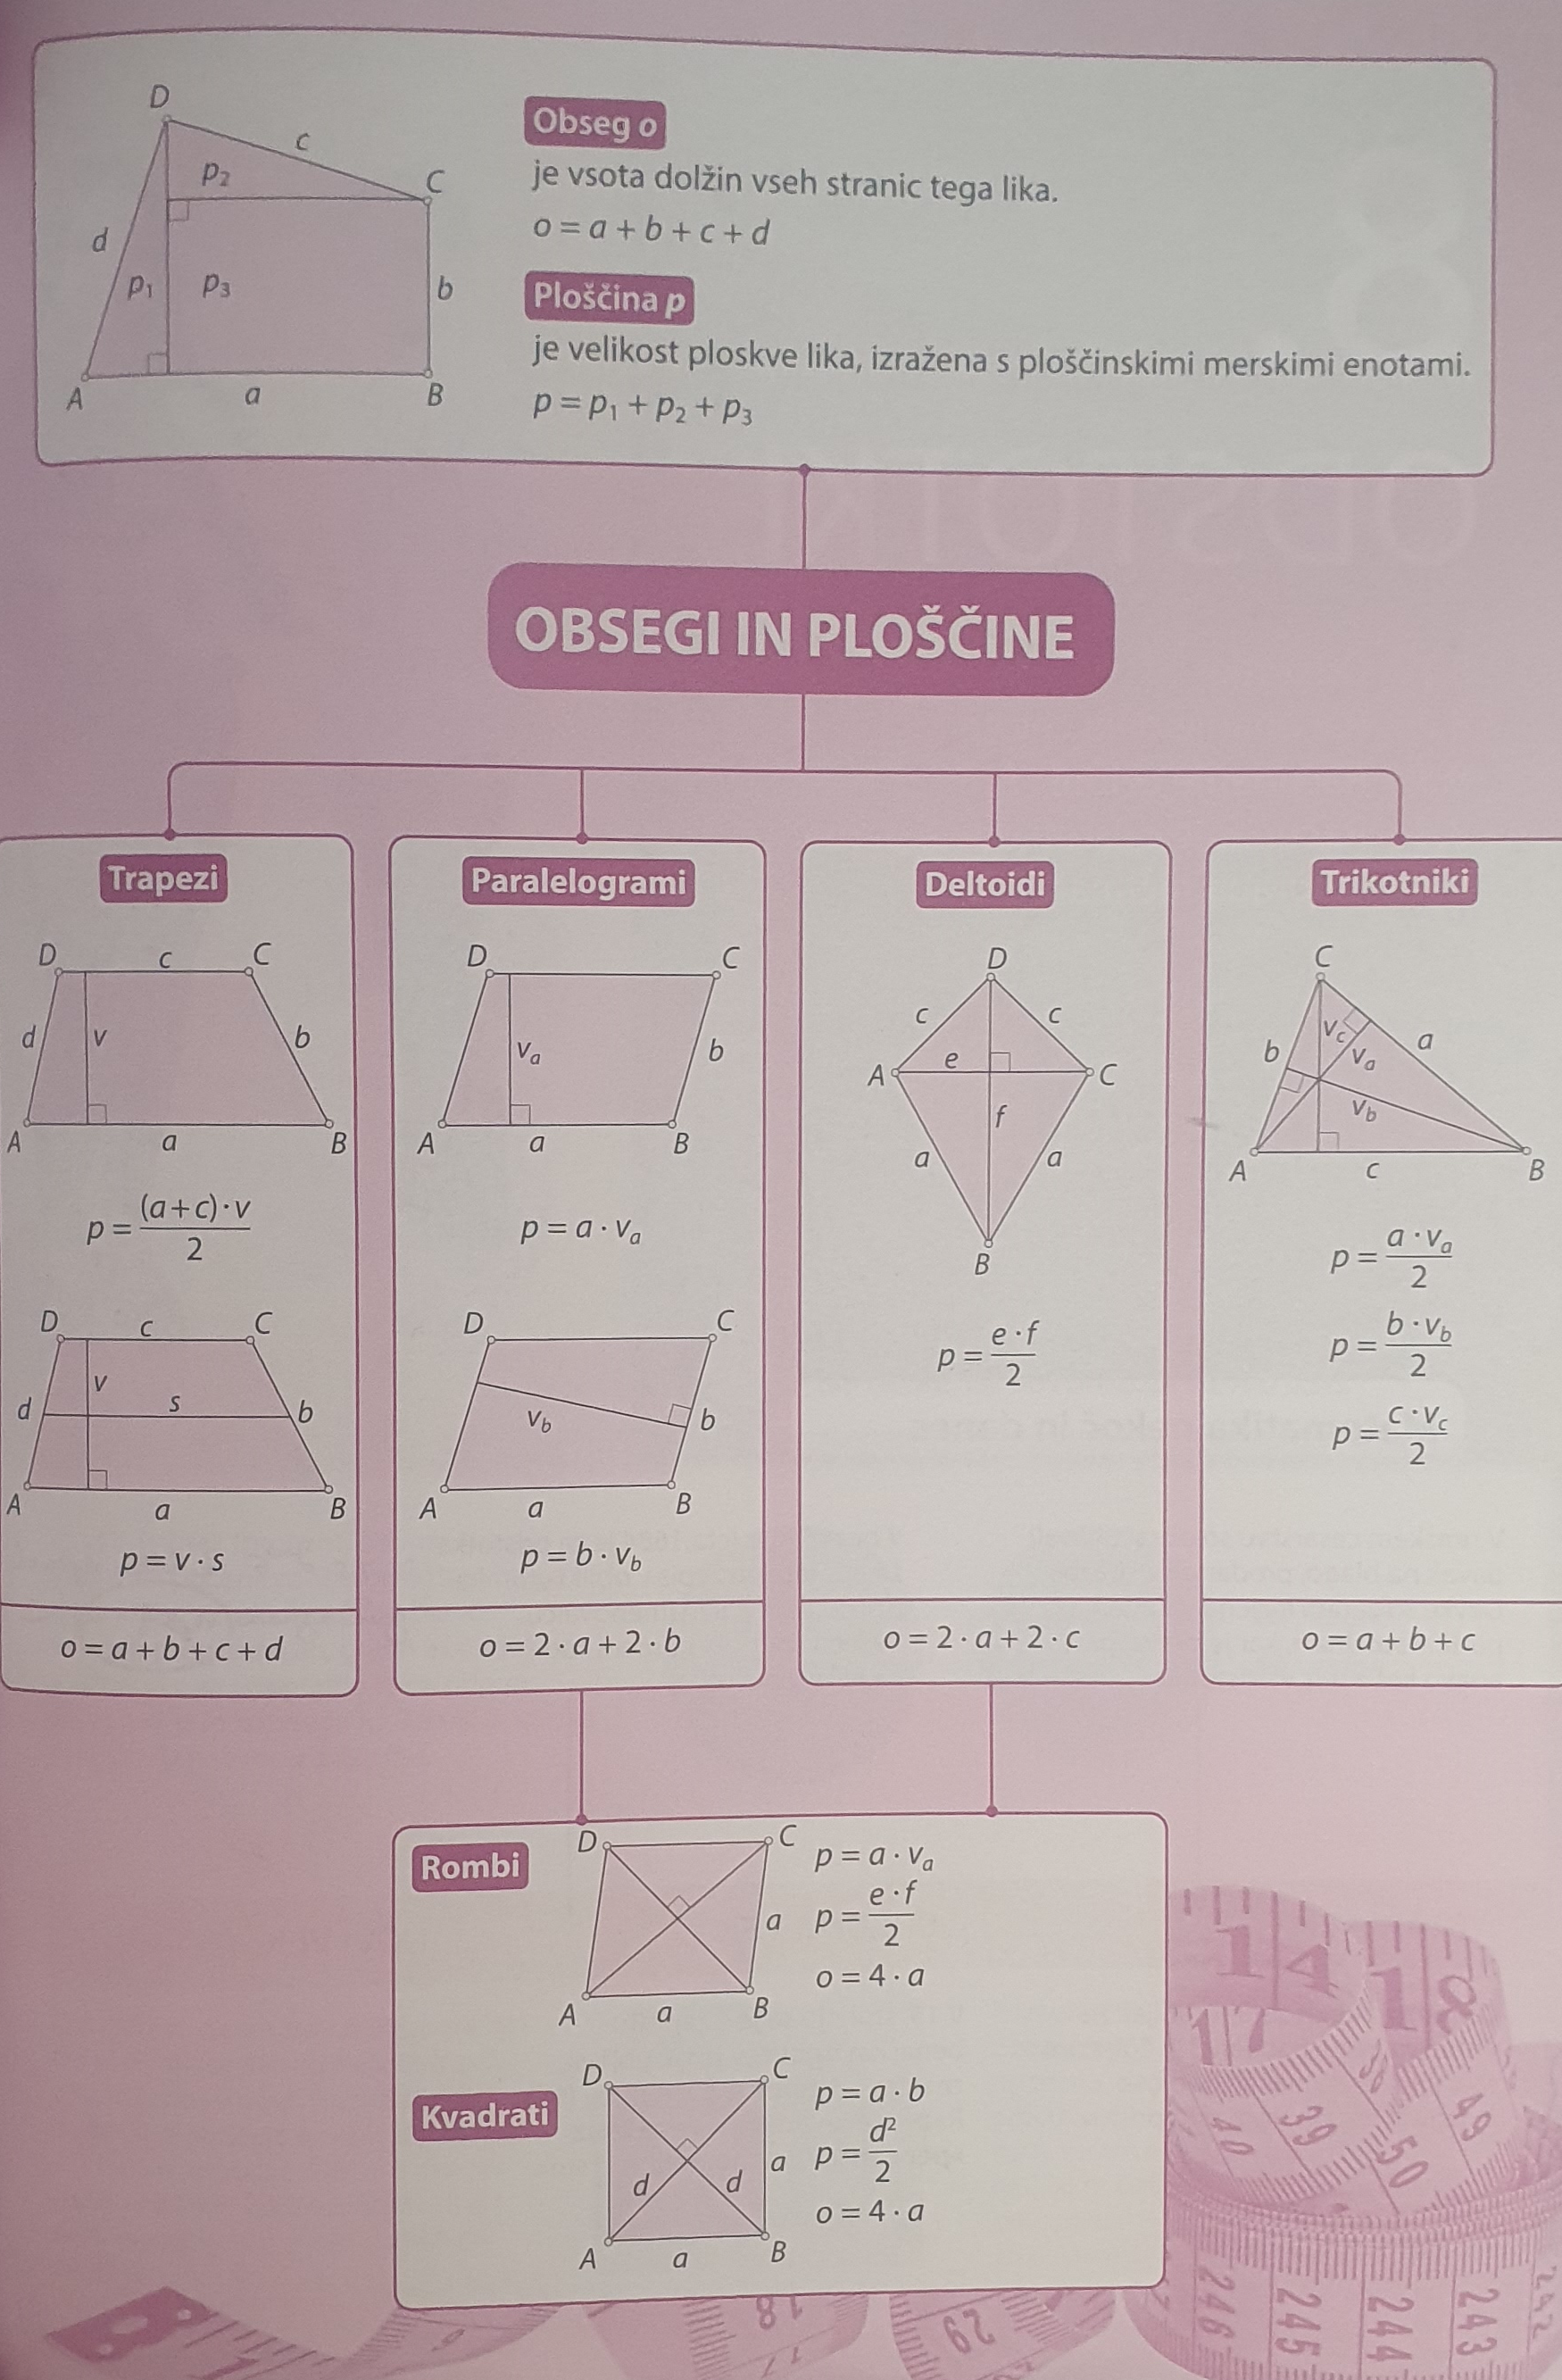
\includegraphics[width=\linewidth]{obsegInPloscinePovzetek.png}
%     \centering
%     % \caption{Izračun ploščine s preoblikovanjem lika v pravokotnik.}
% \end{figure}

\pagebreak
\section{Podatki}
\subsection{Vrste prikazov}

\begin{definicija}
    Podatke lahko predstavimo v obliki različnih prikazov:
    \begin{itemize}
        \item prikaz s preglednico (tabelo),
        \item prikaz s stolpci,
        \item prikaz z vrsticami,
        \item tortni prikaz,
        \item točkovni prikaz,
        \item drevesni prikaz.
    \end{itemize}
\end{definicija}

\begin{figure}[h]
    \includegraphics[width=0.8\linewidth]{prikazi.png}
    \centering
    \caption{Nekaj različnih prikazov.}
\end{figure}
% \begin{figure}[h]
%     \includegraphics[width=0.4\linewidth]{tabela.png}
%     \centering
%     \caption{Preglednica/tabela.}
% \end{figure}
% \begin{figure}[h]
%     \includegraphics[width=0.4\linewidth]{stolpicniPrikaz.png}
%     \centering
%     \caption{Stolpični prikaz.}
% \end{figure}
% \begin{figure}[h]
%     \includegraphics[width=0.4\linewidth]{tockovniPrikaz.png}
%     \centering
%     \caption{Točkovni prikaz.}
% \end{figure}
% \begin{figure}[h]
%     \includegraphics[width=0.4\linewidth]{krozniPrikaz.png}
%     \centering
%     \caption{Tortni prikaz.}
% \end{figure}

\subsection{Drevesni prikaz}

\begin{definicija}[Drevesni prikaz]
    Drevesni prikaz ali kombinatorično drevo je diagram, ki prikaže vse korake odločanja. Kombinatorično štetje je preštevanje vseh mogočih zaporednih odločanj.
\end{definicija}

\begin{figure}[h]
    \includegraphics[width=\linewidth]{drevesniPrikaz.png}
    \centering
    \caption{Drevesni prikaz, ki prikazuje možne izbire kosila (najprej izberemo juho, nato glavno jed in na koncu sladico).}
\end{figure}

Iz prikazane slike je razvidno, da je vseh možnih različnih menijev $4 \cdot 2 \cdot 3 = 24$


\pagebreak
\subsection{Koordinatna mreža}

\begin{definicija}[Koordinatna mreža]
    Lego točke v ravnini natančno opišemo v koordinatni mreži. V koordinatni mreži se pod pravim kotom sekata številski premici: vodoravna os x (abscisa) in navpična os y (ordinata). Lega vsake točke je določena z dvema koordinatam $(x, y)$. Presečišče obeh osi je izhodišče koordinatnega sistema $(0,0)$.
\end{definicija}

\begin{figure}[h]
    \includegraphics[width=0.7\linewidth]{koordinatnaMreza.png}
    \centering
    \caption{Točka A(5, 2) v koordinatni mreži.}
\end{figure}


\pagebreak
\subsection{Medsebojna odvisnost količin}

\begin{definicija}
    Poznamo stalne količne (konstante) in spremenljive količine (spremenljivke). Odvisnost dveh količin lahko prikažemo v koordinatni mreži s točkami, ki so določene z urejenim parom števil (x, y). Spremenljivka x je neodvisna in jo rišemo na vodoravni osi, spremenljivka y pa je odvisna in jo rišemo na navpični osi. Točke prikaza so lahko med seboj nepovezane. Tak prikaz imenjujemo točkovni prikaz, ki pride v poštev tudi pri diskrednih spremenljivkah. Med seboj povezane količine lahko prikažemo s črtnim prikazom - grafom.
\end{definicija}


\begin{figure}[h]
    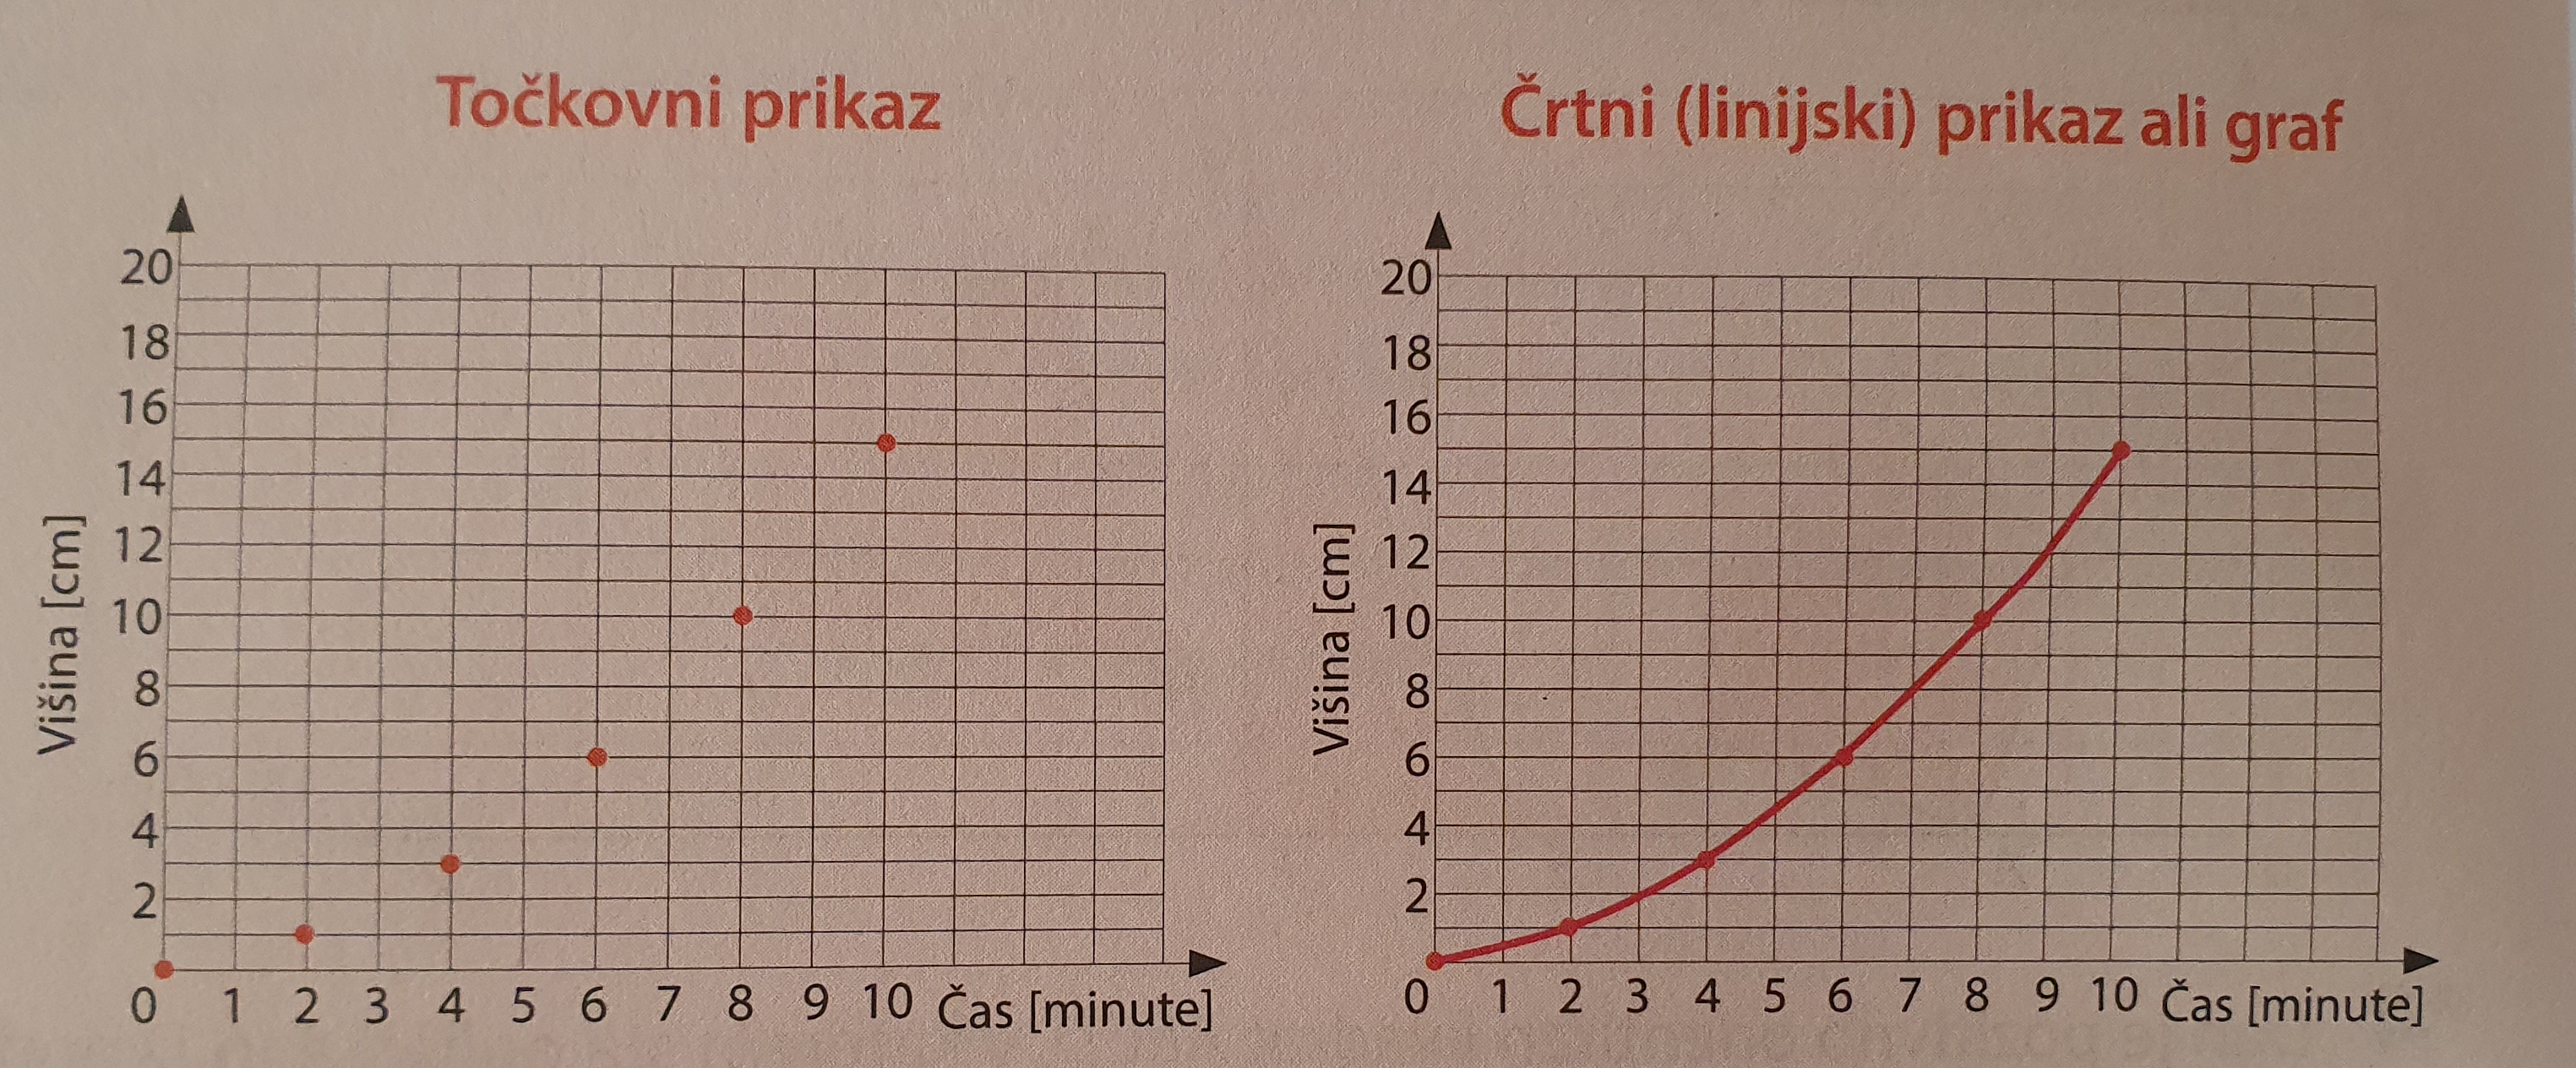
\includegraphics[width=\linewidth]{graf.png}
    \centering
    \caption{Točkovni in črtni prikaz (graf).}
\end{figure}


\pagebreak
\subsection{Aritmetnična srednia}

\begin{definicija}[Aritmetnična sredina]
    Aritmetična sredina ali povprečje $\overline{x}$ je količnik med vsoto vseh vrednosti številskih podatkov in številom vseh podatkov.
    \[
        \overline{x} = \frac{x_1 + x_2 + \dots + x_n}{n}    
    \]
    Aritmetično sredino določamo samo številskim podatkom.
\end{definicija}

\end{document}